
The discussion is based on the motion of two bodies that are subject to conservative, central forces from the other but no other "external" forces. Examples include the motion by gravity in a binary star system or protons and electrons moving in a hydrogen atom.

The center of mass (CM) of a two-body system is defined from the earlier section as:

\begin{equation*}
    \vec{R} = \frac{m_1 \vec{r_1} + m_2 \vec{r_2}}{m_1 + m_2} = \frac{m_1 \vec{r_1} + m_2 \vec{r_2}}{M}
\end{equation*}

\noindent where $M$ is the total mass of the system. Writing the Lagrangian of a system with the generalized coordinates $\vec{R}$ (CM) and $\vec{r}$ (relative position), yields a new constant called the {\bfseries reduced mass}, $\mu = \frac{m_1 m_2}{m_1 + m_2}$. This value is always less than both $m_1$ and $m_2$, but if $m_1 << m_2$ then $\mu \approx m_1$. In the Earth-Sun system, $\mu$ is almost the mass of the Earth. The Lagrangian yields a kinetic energy that involves the relative position and reduced mass, instead of treating both bodies separately.

\begin{equation*}
    \mathcal{L} = T-U = \frac{1}{2}M \vec{\dot{R}}^2 + \frac{1}{2}\mu \vec{\dot{r}}^2 - U(r).
\end{equation*}

The term $\vec{R}$ is considered ignorable here because $\mathcal{L}$ is independent of $\vec{R}$. This is a direct consequence of conservation of total momentum. The only term involving $\vec{R}$ has the form of a Lagrangian of a free particle of mass $M$ and position $\vec{R}$.

The second and third term involving $\vec{r}$ is the Lagrangian for a single particle of mass $\mu$ and position $\vec{r}$ with potential energy $U(r)$. Thus the Lagrangian is Newton's second law of such as particle, $\mu \vec{\ddot{r}} = -\nabla U(\vec{r})$.

The obvious choice of coordinates for the Lagrangian is spherical $(r,\phi)$,

\begin{equation*}
    \mathcal{L} = \frac{1}{2}\mu (\dot{r}^2 + r^2 \dot{\phi}^2) - U(r).
\end{equation*}

Since the Lagrangian is independent of $\phi$, the coordinate $\phi$ is ignorable, and the equation corresponding to $\phi$ is simply, $\frac{\partial \mathcal{L}}{\partial \dot{\phi}} = \mu r^2 \dot{\phi} = const = \ell$. This is the conservation of angular momentum.

On the other hand the {\bfseries radial equation} (the Lagrange equation corresponding to $r$) is,

\begin{equation*}
    \frac{\partial \mathcal{L}}{\partial r} = \frac{d}{dt} \frac{\partial \mathcal{L}}{\partial \dot{r}} \rightarrow \mu r \dot{\phi}^2 - \frac{dU}{dr} = \mu \ddot{r}.
\end{equation*}

The goal is to use the $\phi$ equation (determined by initial conditions) bu putting $\ell$ in the radial equation. To do this, we solve for $\dot{\phi} = \frac{\ell}{\mu r^2}$. Plugging this into the radial equation allows $\ell$ to be used instead. Rewriting the radial equation,

\begin{equation*}
    \mu \ddot{r} = - \frac{dU}{dr} + \mu r \dot{\phi}^2 = - \frac{dU}{dr} + F_{cf}.
\end{equation*}

This is the equation of motion for a particle in {\itshape one} dimension of mass $\mu$ and position $r$, subject to actual force $-\frac{dU}{dr}$ and a fictitious centrifgual force $F_{cf}$. In other words, the particels radial motion is exactly the same as if the particle were moving in one dimension subject to the actual force and centrifugal force labeled above. 

$F_{cf}$ can also be written to remove $\dot{\phi}$, $F_{cf} = \frac{\ell^2}{\mu r^3}$. Expressing this force as a centrifugal potential energy, $F_{cf} = -\frac{dU_{cf}}{dr}$, where $U_{cf}$ is defined as $\frac{\ell^2}{2 \mu r^2}$. Rewriting the radial equation,

\begin{equation*}
    \mu \ddot{r} = -\frac{d}{dr}[U(r) + U_{cf}(r)] - \frac{d}{dr} U_{eff}(r)
\end{equation*}

\noindent where $U_{eff}(r)$ is the {\bfseries effective potential energy}, or the sum of the actual potential energy and the centrifugal potential: $U_{eff}(r) = U(r) + \frac{\ell^2}{2 \mu r^2}$.

To find the details of an orbit (in an inverse square law), you must look closely at the radial equation. We see that $T + U_{eff}(r)$ is actually just the conservation of energy (i.e. $=E$). This idea is shown graphically in figure \ref{fig:Ueff} for a orbiting planetary body such as a comet.


\begin{figure}
    \centering
    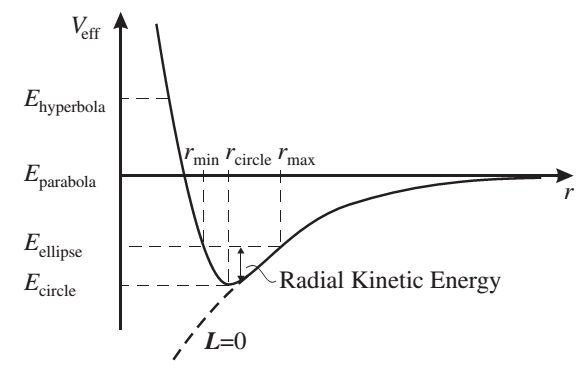
\includegraphics[width=10cm]{Classical_Mechanics/2.15-two-central-forces/Ueff.png}
    \caption{When a comet with $E < 0$ the orbit is {\bfseries bounded} circularly or elliptically. The orbit will oscillate between $r_{min}$ and $r_{max}$ in an elliptical orbit. When $E > 0$, the orbit will be {\bfseries unbounded} and orbit in a hyperbola. [image credit: \href{https://physics.stackexchange.com/questions/379708/doubts-about-the-effective-potential-in-newtonian-gravity}{Stack Overflow}]}
    \label{fig:Ueff}
\end{figure}
